\section{Auswertung}
\label{sec:Auswertung}

\subsection{Reflexionsgesetz}

  Zur Überprüfung des Reflexionsgesetz werden mit einem grünen Laser die Ausfallswinkel für verschiedene Einfallswinkel gemessen, die Daten sind in der 
  \autoref{tab:refl} zu finden. 

  \begin{table}[H]
    \centering
    \caption{Die Messdaten von der Überprüfung des Reflexionsgesetzes.}
    \label{tab:refl}
    \begin{tabular}{S[table-format=2.1] S[table-format=2.1] }
      \toprule
      {Einfallswinkel $\alpha / \si{\degree} $} & {Ausfallswinkel $\beta / \si{\degree} $} \\
      \midrule
      20.0 & 20.0 \\
      30.0 & 30.5 \\
      35.0 & 36.0 \\
      40.0 & 41.0 \\
      50.0 & 51.0 \\
      60.0 & 61.5 \\
      70.0 & 72.0 \\
      \bottomrule 
    \end{tabular}
  \end{table}

  \noindent Die Messdaten werden in einem $\alpha$ - $\beta $ - Diagramm aufgetragen sowie eine lineare Ausgleichsrechung der Form $\beta = A \cdot \alpha + B$. Diese
  wird mit python errechnet und ist in der \autoref{fig:refl} zu sehen. 

  \begin{figure}[H]
    \centering
    \includegraphics[width=\textwidth]{build/reflexion.pdf}
    \caption{Der Plot zur Überprüfung des Reflexionsgesetzes.}
    \label{fig:refl}
  \end{figure}

  \noindent Für die Parameter ergeben sich:
  \begin{align*}
    A &= \num{1.035(5)}\\
    B &= \SI{-0.543(216)}{\degree}
  \end{align*}

\subsection{Brechungsgesetz}\label{subsec:brec}

  Es werden für verschiedene Einfallswinkel $\alpha$  die Brechungswinkel $\beta$ bei einer Brechung in einer Plexiglasplatte gemessen. In der \autoref{tab:brec} 
  sind neben diesen Winkeln der jeweils über das Snellius Brechungsgesetz
  \begin{align*}
    \sin(\alpha) n_1 &= n_2 \sin(\beta) &\iff n &= \frac{\sin(\alpha)}{\sin(\beta)} 
  \end{align*}
  berechnete Brechungsindex von Plexiglas. 

  \begin{table}[H]
    \centering
    \caption{Die gemessenen Winkel und der daraus errechnete Brechungsindex für Plexiglas.}
    \label{tab:brec}
    \begin{tabular}{S[table-format=2.1] S[table-format=2.1] S[table-format=1.3]}
      \toprule
      {$\alpha / \si{\degree} $} & {$\beta / \si{\degree} $} & {$n_{\text{Plexiglas}} $}\\
      \midrule
      20.0 & 14.0 & 1.414 \\
      30.0 & 20.0 & 1.462 \\
      35.0 & 23.0 & 1.468 \\
      40.0 & 26.0 & 1.466 \\
      50.0 & 31.5 & 1.466 \\
      60.0 & 36.0 & 1.473 \\
      70.0 & 39.0 & 1.493 \\
      \bottomrule 
    \end{tabular}
  \end{table}

  \noindent Nun wird für den Brechungsindex von Plexiglas der Mittelwert aus den Werten in \autoref{tab:brec} berechnet: 
  \begin{equation*}
    n_{\text{Plexiglas}} = \num{1.463(8)}
  \end{equation*}
  Die Geschwindigkeit von Licht in den verschiedenen Materialien steht in diesem Zusammenhang mit den Brechungindices
  \begin{equation*}
    \frac{v_1}{v_2} = \frac{n_2}{n_1}.
  \end{equation*}
  Somit lässt sich die Lichtgeschwindigkeit in Plexiglas aus dem ermittelten Brechungsindex berechnen, es folgt
  \begin{equation*}
    v_{\text{Plexiglas}} = \SI{204884121(1181566)}{\metre\per\second}. 
  \end{equation*}

\subsection{Planparallele Platten}

  Zur Bestimmung des Strahlenversatz werden keine neuen Winkel ausgemessen, sondern die Daten der Brechungswinkel aus dem vorherigen Aufgabenteil genutzt.
  In der \autoref{fig:planpar} ist schematisch der Strahlenweg ohne Brechung (gestrichelt) und der mit Brechung an dem Plexiglasquader dargestellt. 
  
  \begin{figure}
    \centering
    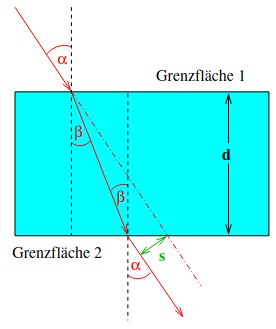
\includegraphics[width=0.4\textwidth]{bilder/planparallel.png}
    \caption{Eine Skizze zum auftretenen Strahlenversatz. \cite{anleitung}}
    \label{fig:planpar}
  \end{figure}

  \noindent Der Strahlenversatz berechnet sich über 
  \begin{equation*}
    s = d \frac{\sin(\alpha - \beta)}{\cos(\beta)}. 
  \end{equation*}
  Nun wird über diese Formel der Strahlenversatz einmal mit den gemessenen Einfalls- und Brechungswinkel berechnet. In einer anderen Methode wird der Winkel $\beta$ 
  aus dem Brechungsgesetz mit dem in \ref{subsec:brec} ermittelten Brechungsindex für Plexiglas errechnet 
  \begin{equation*}
    \beta_2 = \arcsin\left(\frac{\sin(\alpha)}{n_{\text{Plexiglas}}}\right). % unp.arcsin(np.sin(alpha * np.pi /180)/ unp.nominal_values(n)) * 180 / np.pi 
  \end{equation*}
  Mit diesem $\beta_2$ wird dann nochmal der Strahlenversatz ausgerechnet. Die Daten sind in der \autoref{tab:planpar} zu finden. 

  \begin{table}[H]
    \centering
    \caption{Die Werte der Messung bei Brechung und dem daraus gerechneten Strahlungsversatz.}
    \label{tab:planpar}
    \begin{tabular}{S[table-format=2.1] S[table-format=2.1] S[table-format=2.3] S[table-format=2.3] S[table-format=2.3] }
      \toprule
      & \multicolumn{2}{c}{Brechungswinkel} & \multicolumn{2}{c}{Brechungsindex}\\
      \cmidrule(lr){2-3} \cmidrule(lr){4-5}
      {$\alpha / \si{\degree} $} & {$\beta / \si{\degree} $} & {$s_1 / \si{\milli\metre}$}  & {$\beta_2 / \si{\degree} $} & {$s_2 / \si{\milli\metre}$}\\
      \midrule
      20.0 & 14.0 & 6.302 & 13.518 & 6.793 \\
      30.0 & 20.0 & 10.810 & 19.981 & 10.829 \\
      35.0 & 23.0 & 13.213 & 23.079 & 13.136 \\
      40.0 & 26.0 & 15.746 & 26.059 & 15.689 \\
      50.0 & 31.5 & 21.770 & 31.569 & 21.708 \\
      60.0 & 36.0 & 29.411 & 36.289 & 29.185 \\
      70.0 & 39.0 & 38.770 & 39.956 & 38.209 \\
      \bottomrule 
    \end{tabular}
  \end{table}

  \noindent Es ist zu sehen, dass sich die beiden errechneten Werte für den Strahlenversatz für den jeweiligen Einfallswinkel sehr nah beieinander liegen. 

\subsection{Prisma}

  Es werden für den roten und für den grünen Laser jeweils die Einfallswinkel $\alpha_1$ und Ausfallswinkel $\alpha_2$ bei Bestrahlung eines Prismas notiert. 
  In der \autoref{fig:prism} sind die zu nutzenden Winkel bei der Brechung des Lichtstrahls am Prisma sowie die Ablenkung $\delta$ eingezeichnet. 

  \begin{figure}
    \centering
    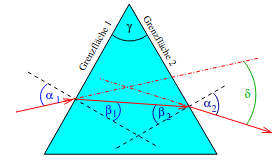
\includegraphics[width=0.4\textwidth]{bilder/prisma.png}
    \caption{Skizze der Strahlengänge im Prisma \cite{anleitung}.}
    \label{fig:prism}
  \end{figure}

  \noindent Die zu betrachtene Ablenkung $\delta$ wird mit 
  \begin{equation*}
    \delta = \left(\alpha_1 + \alpha_2\right) - \left(\beta_1 + \beta_2\right)
  \end{equation*}
  berechnet. Dabei sind die Winkel $\beta_1, \beta_2$ die zu $\alpha_1, \alpha_2$ gehörenden Brechungswinkel. Diese berechnen sich über 
  \begin{equation*}
    \beta_i = \arcsin\left(\frac{\sin(\alpha_i)}{n_{\text{Kronglas}}}\right), 
  \end{equation*}
  da das Prisma aus Kronglas besteht. Außerdem besteht noch die Beziehung $\beta_1 + \beta_2 = \gamma$, wobei $\gamma$ in diesem Fall $\SI{60}{\degree}$ ist. 
  Die aufgenommenen Messdaten und daraus errechneten Werte sind in der \autoref{tab:prismisadancer} zu finden.

  \begin{table}[H]
    \centering
    \caption{Die Messdaten von der Messung mit dem Prisma.}
    \label{tab:prismisadancer}
    \begin{tabular}{S[table-format=2.1] S[table-format=2.3] S[table-format=2.1] S[table-format=2.3] S[table-format=2.3] S[table-format=2.1] S[table-format=2.3] S[table-format=2.3] }
      \toprule
      & & \multicolumn{3}{c}{grüner Laser} & \multicolumn{3}{c}{roter Laser}\\
      \cmidrule(lr){3-5} \cmidrule(lr){6-8}
      {$\alpha_1 / \si{\degree} $} & {$\beta_1 / \si{\degree} $}  & {$\alpha_2 / \si{\degree} $} & {$\beta_2 / \si{\degree} $} &{$\delta / \si{\degree}$} & {$\alpha_2 / \si{\degree} $} & {$\beta_2 / \si{\degree} $} & {$\delta / \si{\degree}$}\\
      \midrule
      30.0 & 20.027 & 78.5 & 42.158 & 46.315 & 78.0 & 42.064 & 45.909 \\
      35.0 & 23.133 & 66.5 & 38.912 & 39.456 & 65.5 & 38.555 & 38.813 \\
      40.0 & 26.121 & 59.0 & 35.952 & 36.928 & 58.0 & 35.511 & 36.368 \\
      50.0 & 31.647 & 47.5 & 30.330 & 35.522 & 47.0 & 30.061 & 35.291 \\
      60.0 & 36.382 & 38.5 & 25.238 & 36.880 & 37.5 & 24.643 & 36.475 \\
      \bottomrule 
    \end{tabular}
  \end{table}

  \noindent Es ist auffällig, dass der Wert für den Einfallswinkel $\alpha_1 = \SI{30}{\degree}$ deutlich größer als die anderen Werte ist. Die Ablenkung ist schon 
  für den wenig größeren Einfallswinkel $\alpha_1 = \SI{35}{\degree}$ deutlich kleiner. Für die Einfallswinkel $\alpha_1 = \SI{40}{\degree}, \SI{50}{\degree}$ und 
  $\SI{60}{\degree}$ sind die Ablenkungen $\delta$ sehr nah beieinander. 

\subsection{Beugung am Gitter}

  Es werden für drei verschiedene Gitter die Winkel der Maxima und deren Ordnung gemessen und notiert. Die Wellenlänge des Lichtes lässt sich durch
  \begin{equation*}
    \lambda = d \frac{\sin(\phi)}{k}
  \end{equation*}
  berechnen, wobei $d$ die Gitterkonstante darstellt und $k$ die Beugungsordnung. Die Daten und daraus errechneten Werte sind in der \autoref{tab:beugunggitter} 
  zu finden.

  \begin{table}[H]
    \centering
    \caption{Die Daten von der Messung von Beugung am Gitter.}
    \label{tab:beugunggitter}
    \begin{tabular}{c S[table-format=1.0] S[table-format=2.1] S[table-format=3.2] S[table-format=2.1] S[table-format=3.2]} 
      \toprule
      & & \multicolumn{2}{c}{grüner Laser} & \multicolumn{2}{c}{roter Laser}\\
      \cmidrule(lr){3-4} \cmidrule(lr){5-6}
      {$d / \si{\micro\metre}$} & {$k$} & {$\phi / \si{\degree} $} & {$\lambda / \si{\nano\metre} $} & {$\phi / \si{\degree} $} & {$\lambda / \si{\nano\metre} $} \\
      \midrule
      $\frac{5}{3}$ & 1 & 19.5 & 556.34 & 23  & 651.22 \\
                    &   & 18   & 515.03 & 22  & 624.34 \\
      \midrule
      $\frac{10}{3}$& 1 & 9.5  & 550.16 & 11  & 636.03 \\
                    &   & 8.5  & 492.70 & 10.5& 607.45 \\
                    & 2 & 19   & 542.61 & 23  & 651.22 \\
                    &   & 17.5 & 501.18 & 21.5& 610.84 \\
                    & 3 & 29   & 538.68 & 35  & 637.31 \\
                    &   & 27.5 & 513.05 &  34 & 621.33 \\
      \midrule
       10           & 1 & 3.5  & 610.49 & 4   & 697.56 \\
                    &   & 2.5  & 436.19 & 3.5 & 610.49 \\
                    & 2 &  7   & 609.35 & 8   & 695.87 \\
                    &   & 5.5  & 479.23 &  7  & 609.35 \\
                    & 3 &  10  & 578.83 &11.5 & 664.56 \\
                    &   & 8.5  & 492.70 &10.5 & 607.45 \\
                    & 4 & 13   & 562.38 & 15.5& 668.10 \\
                    &   & 11.5 & 498.42 & 14.5& 625.95 \\
                    & 5 & 16.5 & 568.03 & 19.5& 667.61 \\
                    &   &  15  & 517.64 &  18 & 618.03 \\
                    & 6 &  19.5& 556.34 & 23.5& 664.58 \\
                    &   &  18  & 515.03 &  22 & 624.34 \\
                    & 7 & 23   & 558.19 & 27.5& 659.64 \\
                    &   & 21.5 & 523.57 &  26 & 626.24 \\
                    & 8 & 26.5 & 557.75 &  32 & 662.40 \\
                    &   & 24.5 & 518.37 &  30 & 625.00 \\
                    & 9 & 30   & 555.56 &     & \\
                    &   &  28  & 521.64 &     & \\
      \bottomrule 
    \end{tabular}
  \end{table}

  \noindent Die experimentell ermittelte Wellenlänge für den jeweiligen Laser ergibt sich aus dem Mittelwert der berechneten Werte in \autoref{tab:beugunggitter}:
  \begin{align*}
    \lambda_{\text{grün}} &= \SI{533(8)}{\nano\metre}\\
    \lambda_{\text{rot}}  &= \SI{640(5)}{\nano\metre}
  \end{align*}